% Created by tikzDevice version 0.11 on 2018-09-25 14:29:31
% !TEX encoding = UTF-8 Unicode
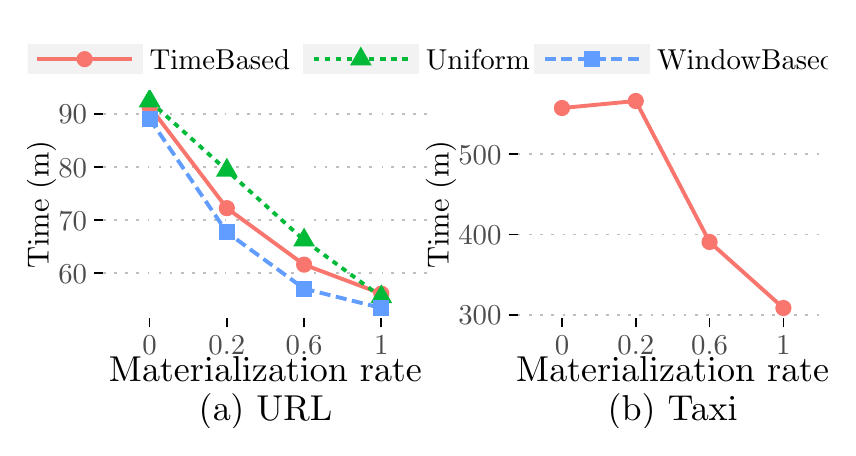
\begin{tikzpicture}[x=1pt,y=1pt]
\definecolor{fillColor}{RGB}{255,255,255}
\path[use as bounding box,fill=fillColor,fill opacity=0.00] (0,0) rectangle (289.08,144.54);
\begin{scope}
\path[clip] (  0.00,  0.00) rectangle (289.08,144.54);
\definecolor{fillColor}{RGB}{255,255,255}

\path[fill=fillColor] (-10.79,121.78) rectangle (299.87,144.54);
\end{scope}
\begin{scope}
\path[clip] (  0.00,  0.00) rectangle (289.08,144.54);
\definecolor{drawColor}{RGB}{255,255,255}
\definecolor{fillColor}{gray}{0.95}

\path[draw=drawColor,line width= 0.6pt,line join=round,line cap=round,fill=fillColor] ( -0.76,127.47) rectangle ( 41.92,138.85);
\end{scope}
\begin{scope}
\path[clip] (  0.00,  0.00) rectangle (289.08,144.54);
\definecolor{drawColor}{RGB}{248,118,109}

\path[draw=drawColor,line width= 1.4pt,line join=round] (  3.50,133.16) -- ( 37.65,133.16);
\end{scope}
\begin{scope}
\path[clip] (  0.00,  0.00) rectangle (289.08,144.54);
\definecolor{fillColor}{RGB}{248,118,109}

\path[fill=fillColor] ( 20.58,133.16) circle (  2.93);
\end{scope}
\begin{scope}
\path[clip] (  0.00,  0.00) rectangle (289.08,144.54);
\definecolor{drawColor}{RGB}{255,255,255}
\definecolor{fillColor}{gray}{0.95}

\path[draw=drawColor,line width= 0.6pt,line join=round,line cap=round,fill=fillColor] ( 99.05,127.47) rectangle (141.73,138.85);
\end{scope}
\begin{scope}
\path[clip] (  0.00,  0.00) rectangle (289.08,144.54);
\definecolor{drawColor}{RGB}{0,186,56}

\path[draw=drawColor,line width= 1.4pt,dash pattern=on 2pt off 2pt ,line join=round] (103.32,133.16) -- (137.46,133.16);
\end{scope}
\begin{scope}
\path[clip] (  0.00,  0.00) rectangle (289.08,144.54);
\definecolor{fillColor}{RGB}{0,186,56}

\path[fill=fillColor] (120.39,137.71) --
	(124.33,130.88) --
	(116.45,130.88) --
	cycle;
\end{scope}
\begin{scope}
\path[clip] (  0.00,  0.00) rectangle (289.08,144.54);
\definecolor{drawColor}{RGB}{255,255,255}
\definecolor{fillColor}{gray}{0.95}

\path[draw=drawColor,line width= 0.6pt,line join=round,line cap=round,fill=fillColor] (182.61,127.47) rectangle (225.28,138.85);
\end{scope}
\begin{scope}
\path[clip] (  0.00,  0.00) rectangle (289.08,144.54);
\definecolor{drawColor}{RGB}{97,156,255}

\path[draw=drawColor,line width= 1.4pt,dash pattern=on 4pt off 2pt ,line join=round] (186.87,133.16) -- (221.02,133.16);
\end{scope}
\begin{scope}
\path[clip] (  0.00,  0.00) rectangle (289.08,144.54);
\definecolor{fillColor}{RGB}{97,156,255}

\path[fill=fillColor] (201.02,130.23) --
	(206.87,130.23) --
	(206.87,136.08) --
	(201.02,136.08) --
	cycle;
\end{scope}
\begin{scope}
\path[clip] (  0.00,  0.00) rectangle (289.08,144.54);
\definecolor{drawColor}{RGB}{0,0,0}

\node[text=drawColor,anchor=base west,inner sep=0pt, outer sep=0pt, scale=  1.04] at ( 44.08,129.58) {TimeBased};
\end{scope}
\begin{scope}
\path[clip] (  0.00,  0.00) rectangle (289.08,144.54);
\definecolor{drawColor}{RGB}{0,0,0}

\node[text=drawColor,anchor=base west,inner sep=0pt, outer sep=0pt, scale=  1.04] at (143.90,129.58) {Uniform};
\end{scope}
\begin{scope}
\path[clip] (  0.00,  0.00) rectangle (289.08,144.54);
\definecolor{drawColor}{RGB}{0,0,0}

\node[text=drawColor,anchor=base west,inner sep=0pt, outer sep=0pt, scale=  1.04] at (227.45,129.58) {WindowBased};
\end{scope}
\begin{scope}
\path[clip] (  0.00,  0.00) rectangle (144.54,121.78);
\definecolor{drawColor}{RGB}{255,255,255}
\definecolor{fillColor}{RGB}{255,255,255}

\path[draw=drawColor,line width= 0.6pt,line join=round,line cap=round,fill=fillColor] (  0.00,  0.00) rectangle (144.54,121.78);
\end{scope}
\begin{scope}
\path[clip] ( 27.32, 39.50) rectangle (144.54,121.78);
\definecolor{fillColor}{RGB}{255,255,255}

\path[fill=fillColor] ( 27.32, 39.50) rectangle (144.54,121.78);
\definecolor{drawColor}{RGB}{255,255,255}

\path[draw=drawColor,line width= 0.3pt,line join=round] ( 27.32, 46.22) --
	(144.54, 46.22);

\path[draw=drawColor,line width= 0.3pt,line join=round] ( 27.32, 65.40) --
	(144.54, 65.40);

\path[draw=drawColor,line width= 0.3pt,line join=round] ( 27.32, 84.57) --
	(144.54, 84.57);

\path[draw=drawColor,line width= 0.3pt,line join=round] ( 27.32,103.75) --
	(144.54,103.75);
\definecolor{drawColor}{RGB}{190,190,190}

\path[draw=drawColor,line width= 0.6pt,dash pattern=on 1pt off 3pt ,line join=round] ( 27.32, 55.81) --
	(144.54, 55.81);

\path[draw=drawColor,line width= 0.6pt,dash pattern=on 1pt off 3pt ,line join=round] ( 27.32, 74.98) --
	(144.54, 74.98);

\path[draw=drawColor,line width= 0.6pt,dash pattern=on 1pt off 3pt ,line join=round] ( 27.32, 94.16) --
	(144.54, 94.16);

\path[draw=drawColor,line width= 0.6pt,dash pattern=on 1pt off 3pt ,line join=round] ( 27.32,113.33) --
	(144.54,113.33);
\definecolor{drawColor}{RGB}{255,255,255}

\path[draw=drawColor,line width= 0.6pt,line join=round] ( 44.06, 39.50) --
	( 44.06,121.78);

\path[draw=drawColor,line width= 0.6pt,line join=round] ( 71.97, 39.50) --
	( 71.97,121.78);

\path[draw=drawColor,line width= 0.6pt,line join=round] ( 99.88, 39.50) --
	( 99.88,121.78);

\path[draw=drawColor,line width= 0.6pt,line join=round] (127.79, 39.50) --
	(127.79,121.78);
\definecolor{drawColor}{RGB}{248,118,109}

\path[draw=drawColor,line width= 1.4pt,line join=round] ( 44.06,116.01) --
	( 71.97, 79.32) --
	( 99.88, 58.91) --
	(127.79, 48.42);
\definecolor{drawColor}{RGB}{0,186,56}

\path[draw=drawColor,line width= 1.4pt,dash pattern=on 2pt off 2pt ,line join=round] ( 44.06,118.04) --
	( 71.97, 92.97) --
	( 99.88, 67.75) --
	(127.79, 47.24);
\definecolor{drawColor}{RGB}{97,156,255}

\path[draw=drawColor,line width= 1.4pt,dash pattern=on 4pt off 2pt ,line join=round] ( 44.06,111.65) --
	( 71.97, 70.61) --
	( 99.88, 50.23) --
	(127.79, 43.24);
\definecolor{fillColor}{RGB}{248,118,109}

\path[fill=fillColor] ( 44.06,116.01) circle (  2.93);

\path[fill=fillColor] ( 71.97, 79.32) circle (  2.93);

\path[fill=fillColor] ( 99.88, 58.91) circle (  2.93);

\path[fill=fillColor] (127.79, 48.42) circle (  2.93);
\definecolor{fillColor}{RGB}{0,186,56}

\path[fill=fillColor] ( 44.06,122.59) --
	( 48.00,115.76) --
	( 40.12,115.76) --
	cycle;

\path[fill=fillColor] ( 71.97, 97.52) --
	( 75.91, 90.69) --
	( 68.03, 90.69) --
	cycle;

\path[fill=fillColor] ( 99.88, 72.30) --
	(103.82, 65.48) --
	( 95.94, 65.48) --
	cycle;

\path[fill=fillColor] (127.79, 51.79) --
	(131.73, 44.97) --
	(123.85, 44.97) --
	cycle;
\definecolor{fillColor}{RGB}{97,156,255}

\path[fill=fillColor] ( 41.14,108.72) --
	( 46.99,108.72) --
	( 46.99,114.57) --
	( 41.14,114.57) --
	cycle;

\path[fill=fillColor] ( 69.05, 67.68) --
	( 74.90, 67.68) --
	( 74.90, 73.53) --
	( 69.05, 73.53) --
	cycle;

\path[fill=fillColor] ( 96.96, 47.30) --
	(102.81, 47.30) --
	(102.81, 53.15) --
	( 96.96, 53.15) --
	cycle;

\path[fill=fillColor] (124.87, 40.31) --
	(130.72, 40.31) --
	(130.72, 46.17) --
	(124.87, 46.17) --
	cycle;
\end{scope}
\begin{scope}
\path[clip] (  0.00,  0.00) rectangle (289.08,144.54);
\definecolor{drawColor}{gray}{0.30}

\node[text=drawColor,anchor=base east,inner sep=0pt, outer sep=0pt, scale=  1.04] at ( 21.47, 52.23) {60};

\node[text=drawColor,anchor=base east,inner sep=0pt, outer sep=0pt, scale=  1.04] at ( 21.47, 71.40) {70};

\node[text=drawColor,anchor=base east,inner sep=0pt, outer sep=0pt, scale=  1.04] at ( 21.47, 90.58) {80};

\node[text=drawColor,anchor=base east,inner sep=0pt, outer sep=0pt, scale=  1.04] at ( 21.47,109.75) {90};
\end{scope}
\begin{scope}
\path[clip] (  0.00,  0.00) rectangle (289.08,144.54);
\definecolor{drawColor}{RGB}{0,0,0}

\path[draw=drawColor,line width= 0.6pt,line join=round] ( 24.07, 55.81) --
	( 27.32, 55.81);

\path[draw=drawColor,line width= 0.6pt,line join=round] ( 24.07, 74.98) --
	( 27.32, 74.98);

\path[draw=drawColor,line width= 0.6pt,line join=round] ( 24.07, 94.16) --
	( 27.32, 94.16);

\path[draw=drawColor,line width= 0.6pt,line join=round] ( 24.07,113.33) --
	( 27.32,113.33);
\end{scope}
\begin{scope}
\path[clip] (  0.00,  0.00) rectangle (289.08,144.54);
\definecolor{drawColor}{RGB}{0,0,0}

\path[draw=drawColor,line width= 0.6pt,line join=round] ( 44.06, 36.25) --
	( 44.06, 39.50);

\path[draw=drawColor,line width= 0.6pt,line join=round] ( 71.97, 36.25) --
	( 71.97, 39.50);

\path[draw=drawColor,line width= 0.6pt,line join=round] ( 99.88, 36.25) --
	( 99.88, 39.50);

\path[draw=drawColor,line width= 0.6pt,line join=round] (127.79, 36.25) --
	(127.79, 39.50);
\end{scope}
\begin{scope}
\path[clip] (  0.00,  0.00) rectangle (289.08,144.54);
\definecolor{drawColor}{gray}{0.30}

\node[text=drawColor,anchor=base,inner sep=0pt, outer sep=0pt, scale=  1.04] at ( 44.06, 26.49) {0};

\node[text=drawColor,anchor=base,inner sep=0pt, outer sep=0pt, scale=  1.04] at ( 71.97, 26.49) {0.2};

\node[text=drawColor,anchor=base,inner sep=0pt, outer sep=0pt, scale=  1.04] at ( 99.88, 26.49) {0.6};

\node[text=drawColor,anchor=base,inner sep=0pt, outer sep=0pt, scale=  1.04] at (127.79, 26.49) {1};
\end{scope}
\begin{scope}
\path[clip] (  0.00,  0.00) rectangle (289.08,144.54);
\definecolor{drawColor}{RGB}{0,0,0}

\node[text=drawColor,anchor=base,inner sep=0pt, outer sep=0pt, scale=  1.30] at ( 85.93, 16.53) {Materialization rate};

\node[text=drawColor,anchor=base,inner sep=0pt, outer sep=0pt, scale=  1.30] at ( 85.93,  2.49) { (a) URL};
\end{scope}
\begin{scope}
\path[clip] (  0.00,  0.00) rectangle (289.08,144.54);
\definecolor{drawColor}{RGB}{0,0,0}

\node[text=drawColor,rotate= 90.00,anchor=base,inner sep=0pt, outer sep=0pt, scale=  1.10] at (  7.58, 80.64) {Time (m)};
\end{scope}
\begin{scope}
\path[clip] (144.54,  0.00) rectangle (289.08,121.78);
\definecolor{drawColor}{RGB}{255,255,255}
\definecolor{fillColor}{RGB}{255,255,255}

\path[draw=drawColor,line width= 0.6pt,line join=round,line cap=round,fill=fillColor] (144.54,  0.00) rectangle (289.08,121.78);
\end{scope}
\begin{scope}
\path[clip] (177.06, 39.50) rectangle (289.08,121.78);
\definecolor{fillColor}{RGB}{255,255,255}

\path[fill=fillColor] (177.06, 39.50) rectangle (289.08,121.78);
\definecolor{drawColor}{RGB}{255,255,255}

\path[draw=drawColor,line width= 0.3pt,line join=round] (177.06, 55.29) --
	(289.08, 55.29);

\path[draw=drawColor,line width= 0.3pt,line join=round] (177.06, 84.30) --
	(289.08, 84.30);

\path[draw=drawColor,line width= 0.3pt,line join=round] (177.06,113.30) --
	(289.08,113.30);
\definecolor{drawColor}{RGB}{190,190,190}

\path[draw=drawColor,line width= 0.6pt,dash pattern=on 1pt off 3pt ,line join=round] (177.06, 40.79) --
	(289.08, 40.79);

\path[draw=drawColor,line width= 0.6pt,dash pattern=on 1pt off 3pt ,line join=round] (177.06, 69.79) --
	(289.08, 69.79);

\path[draw=drawColor,line width= 0.6pt,dash pattern=on 1pt off 3pt ,line join=round] (177.06, 98.80) --
	(289.08, 98.80);
\definecolor{drawColor}{RGB}{255,255,255}

\path[draw=drawColor,line width= 0.6pt,line join=round] (193.06, 39.50) --
	(193.06,121.78);

\path[draw=drawColor,line width= 0.6pt,line join=round] (219.73, 39.50) --
	(219.73,121.78);

\path[draw=drawColor,line width= 0.6pt,line join=round] (246.40, 39.50) --
	(246.40,121.78);

\path[draw=drawColor,line width= 0.6pt,line join=round] (273.08, 39.50) --
	(273.08,121.78);
\definecolor{drawColor}{RGB}{248,118,109}

\path[draw=drawColor,line width= 1.4pt,line join=round] (193.06,115.50) --
	(219.73,118.04) --
	(246.40, 67.10) --
	(273.08, 43.24);
\definecolor{fillColor}{RGB}{248,118,109}

\path[fill=fillColor] (193.06,115.50) circle (  2.93);

\path[fill=fillColor] (219.73,118.04) circle (  2.93);

\path[fill=fillColor] (246.40, 67.10) circle (  2.93);

\path[fill=fillColor] (273.08, 43.24) circle (  2.93);
\end{scope}
\begin{scope}
\path[clip] (  0.00,  0.00) rectangle (289.08,144.54);
\definecolor{drawColor}{gray}{0.30}

\node[text=drawColor,anchor=base east,inner sep=0pt, outer sep=0pt, scale=  1.04] at (171.21, 37.21) {300};

\node[text=drawColor,anchor=base east,inner sep=0pt, outer sep=0pt, scale=  1.04] at (171.21, 66.21) {400};

\node[text=drawColor,anchor=base east,inner sep=0pt, outer sep=0pt, scale=  1.04] at (171.21, 95.22) {500};
\end{scope}
\begin{scope}
\path[clip] (  0.00,  0.00) rectangle (289.08,144.54);
\definecolor{drawColor}{RGB}{0,0,0}

\path[draw=drawColor,line width= 0.6pt,line join=round] (173.81, 40.79) --
	(177.06, 40.79);

\path[draw=drawColor,line width= 0.6pt,line join=round] (173.81, 69.79) --
	(177.06, 69.79);

\path[draw=drawColor,line width= 0.6pt,line join=round] (173.81, 98.80) --
	(177.06, 98.80);
\end{scope}
\begin{scope}
\path[clip] (  0.00,  0.00) rectangle (289.08,144.54);
\definecolor{drawColor}{RGB}{0,0,0}

\path[draw=drawColor,line width= 0.6pt,line join=round] (193.06, 36.25) --
	(193.06, 39.50);

\path[draw=drawColor,line width= 0.6pt,line join=round] (219.73, 36.25) --
	(219.73, 39.50);

\path[draw=drawColor,line width= 0.6pt,line join=round] (246.40, 36.25) --
	(246.40, 39.50);

\path[draw=drawColor,line width= 0.6pt,line join=round] (273.08, 36.25) --
	(273.08, 39.50);
\end{scope}
\begin{scope}
\path[clip] (  0.00,  0.00) rectangle (289.08,144.54);
\definecolor{drawColor}{gray}{0.30}

\node[text=drawColor,anchor=base,inner sep=0pt, outer sep=0pt, scale=  1.04] at (193.06, 26.49) {0};

\node[text=drawColor,anchor=base,inner sep=0pt, outer sep=0pt, scale=  1.04] at (219.73, 26.49) {0.2};

\node[text=drawColor,anchor=base,inner sep=0pt, outer sep=0pt, scale=  1.04] at (246.40, 26.49) {0.6};

\node[text=drawColor,anchor=base,inner sep=0pt, outer sep=0pt, scale=  1.04] at (273.08, 26.49) {1};
\end{scope}
\begin{scope}
\path[clip] (  0.00,  0.00) rectangle (289.08,144.54);
\definecolor{drawColor}{RGB}{0,0,0}

\node[text=drawColor,anchor=base,inner sep=0pt, outer sep=0pt, scale=  1.30] at (233.07, 16.53) {Materialization rate};

\node[text=drawColor,anchor=base,inner sep=0pt, outer sep=0pt, scale=  1.30] at (233.07,  2.49) { (b) Taxi};
\end{scope}
\begin{scope}
\path[clip] (  0.00,  0.00) rectangle (289.08,144.54);
\definecolor{drawColor}{RGB}{0,0,0}

\node[text=drawColor,rotate= 90.00,anchor=base,inner sep=0pt, outer sep=0pt, scale=  1.10] at (152.12, 80.64) {Time (m)};
\end{scope}
\end{tikzpicture}
